\begin{figure}[H]
    \centering
    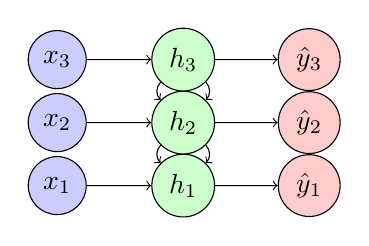
\begin{tikzpicture}[scale=0.8]
        \foreach \t in {1,2,3} {
            \node[circle, draw, fill=blue!20] (X\t) at (0,\t) {$x_\t$};
            \node[circle, draw, fill=green!20] (H\t) at (2,\t) {$h_\t$};
            \node[circle, draw, fill=red!20] (Y\t) at (4,\t) {$\hat{y}_\t$};
            \draw[->] (X\t) -- (H\t);
            \draw[->] (H\t) -- (Y\t);
            \ifnum\t>1
                \draw[->] (H\t) to[bend left=45] (H\the\numexpr\t-1\relax);
                \draw[->] (H\t) to[bend right=45] (H\the\numexpr\t-1\relax);
            \fi
        }
    \end{tikzpicture}
    \caption{Recurrent Neural Network (RNN) unrolled through time.}
    \label{fig:rnn}
\end{figure}